% Chapter Template

\chapter{Extracting insights from Relational Data} % Main chapter title

\label{Chapter4} % Change X to a consecutive number; for referencing this chapter elsewhere, use \ref{ChapterX}

\lhead{Chapter 4. \emph{Extracting insights from Relational Data}} % Change X to a consecutive number; this is for the header on each page - perhaps a shortened title

%----------------------------------------------------------------------------------------
%	SECTION 1
%----------------------------------------------------------------------------------------

\section{Description of Methodology}

The relational schema available for each collection trace and the meaning of each of the fields collected has been described in \ref{Chapter3}.
In this section, the various preprocessing done on each scenario so as to derive useful quantities for visualizing the network and understanding
what exactly is happening in the network is described. All preprocessing code <Pending link to preprocess.py on github> is written in Python3
and the mysql.connector library is used for communication with the MySQL database.
\newline
We describe how to derive three quantities from the existing schema described earlier. The usefulness of these quantities will be shown in Chapter 5.

\begin{itemize}
    \item Time Series of relative ratio of packets in queue for each flow (as defined by source IP) in each switch in the network.
    \item Ingress throughput for each flow in each switch in the network.
    \item Egress throughput for every link as seen in the network.
\end{itemize}

\section{Time Series of relative ratio of packets in queue for each flow}

\subsection{Motivation}
This quantity helps to understand the composition of the queue in a switch at any point in time. By composition, we mean that if, at a point \emph{t} in time,
the size of the queue in a switch is \emph{S} packets, and the number of packets of a flow \emph{i} is \emph{n}, then our plan is to compute \emph{n} / \emph{S} for all flows
at evenly spaced points of time. We do this for all switches. Having a plot of this quantity will help us understand how the distribution of a queue changes as packets arrive
and leave the queue.

\subsection{Computation}
We use the following process for computing the quantity described above.

\begin{enumerate}
    \item Select an interval I which will serve as the gap between successful computations of the relative ratios.
    \item For a point in time \emph{Tcurrent}, perform the following query on the Packetrecords table.
    \begin{verbatim}
    SELECT source_ip, COUNT(hash) 
    FROM packetrecords
    WHERE time_in < Tcurrent AND time_out > Tcurrent
    GROUP BY source_ip;
    \end{verbatim}
    \item This query returns to us the list of flows inside the queue of a switch at a particular time Tcurrent (as ensured by the WHERE clause) as well as the number of packets of
    each flow. The ratios can then be obtained by taking the sum of the packets and dividing each flows number of packets by the total number just computed.
    \item This query is then repeated at every I spaced interval (by incrementing Tcurrent by I each time) in the duration of the records of the switch.
\end{enumerate}

\subsection{Visual Result}
To show how a quantity like this will be helpful, refer to Fig. \ref{fig:QDSimple} where the queue depth has been plotted. The queue depth on it's own does not give us much information on what happened
in the switch, but the composition of the queue (Fig. \ref{fig:QDRatio} (using the relative ratio quantity computed above) gives us a much more revealing insight into how the queue built up over time.
We can clearly understand that the flow coloured in blue is the dominant flow in the queue and is probably a heavy hitter flow. Also refer to Fig. \ref{fig:QDAbsolute} where the absolute relative ratio
of flows has been plotted against time.

\begin{figure}[htbp]
	\centering
		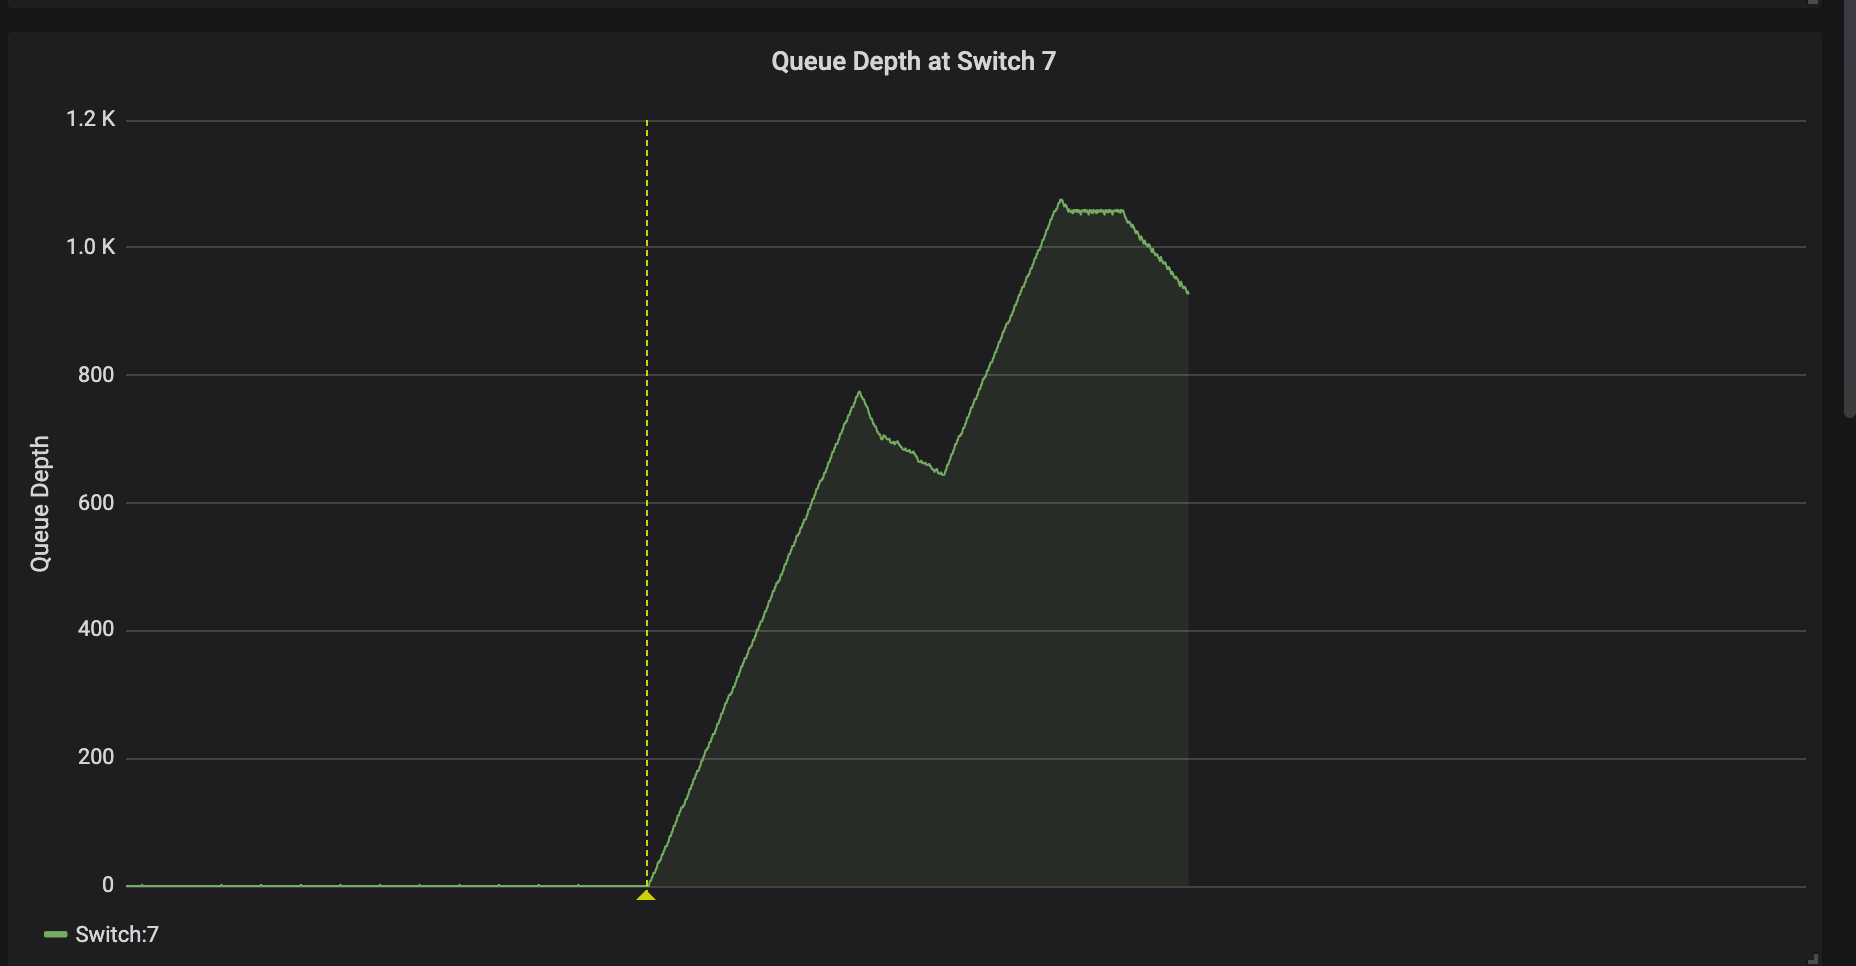
\includegraphics[width=1.0\columnwidth]{Figures/queue_depth_simple.png}
		\rule{35em}{0.5pt}
	\caption[Queue Depth Simple]{Queue Depth at a switch}
	\label{fig:QDSimple}
\end{figure}

\begin{figure}[htbp]
	\centering
		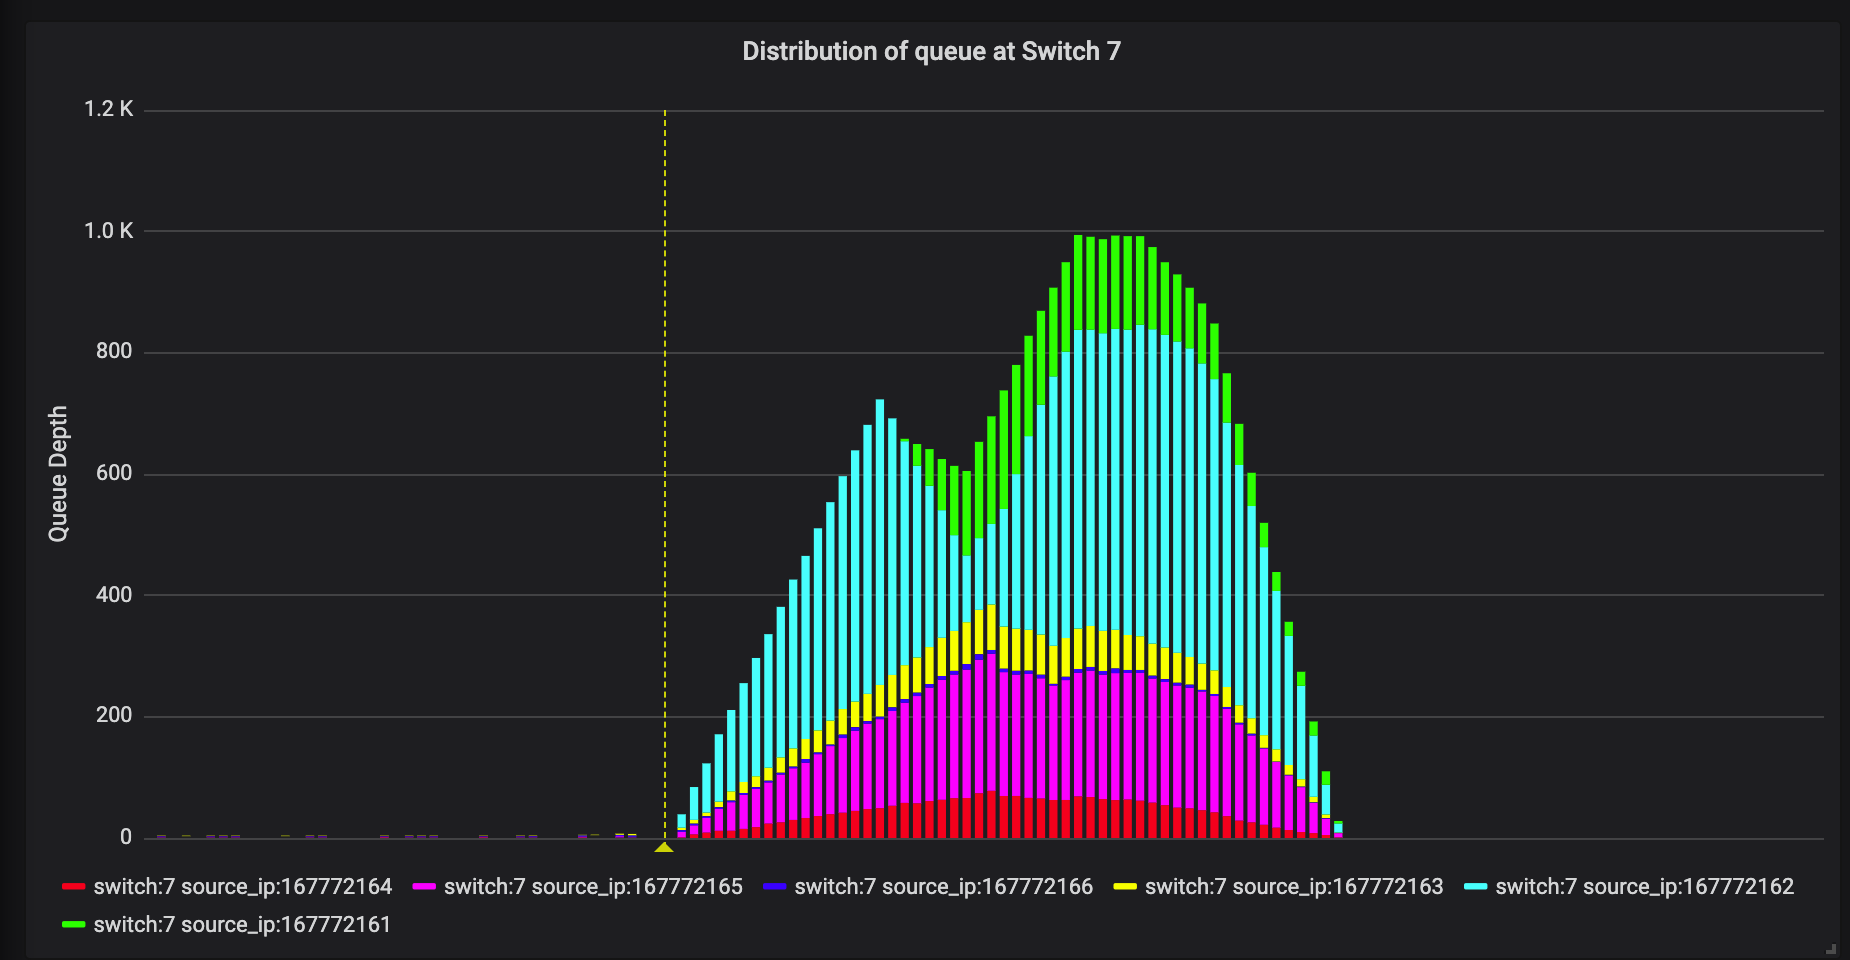
\includegraphics[width=1.0\columnwidth]{Figures/queue_depth_composition.png}
		\rule{35em}{0.5pt}
	\caption[Queue Depth composition]{Queue Depth composition at a switch. Each colour represents packets from one particular flow / source IP}
	\label{fig:QDRatio}
\end{figure}

\begin{figure}[htbp]
	\centering
		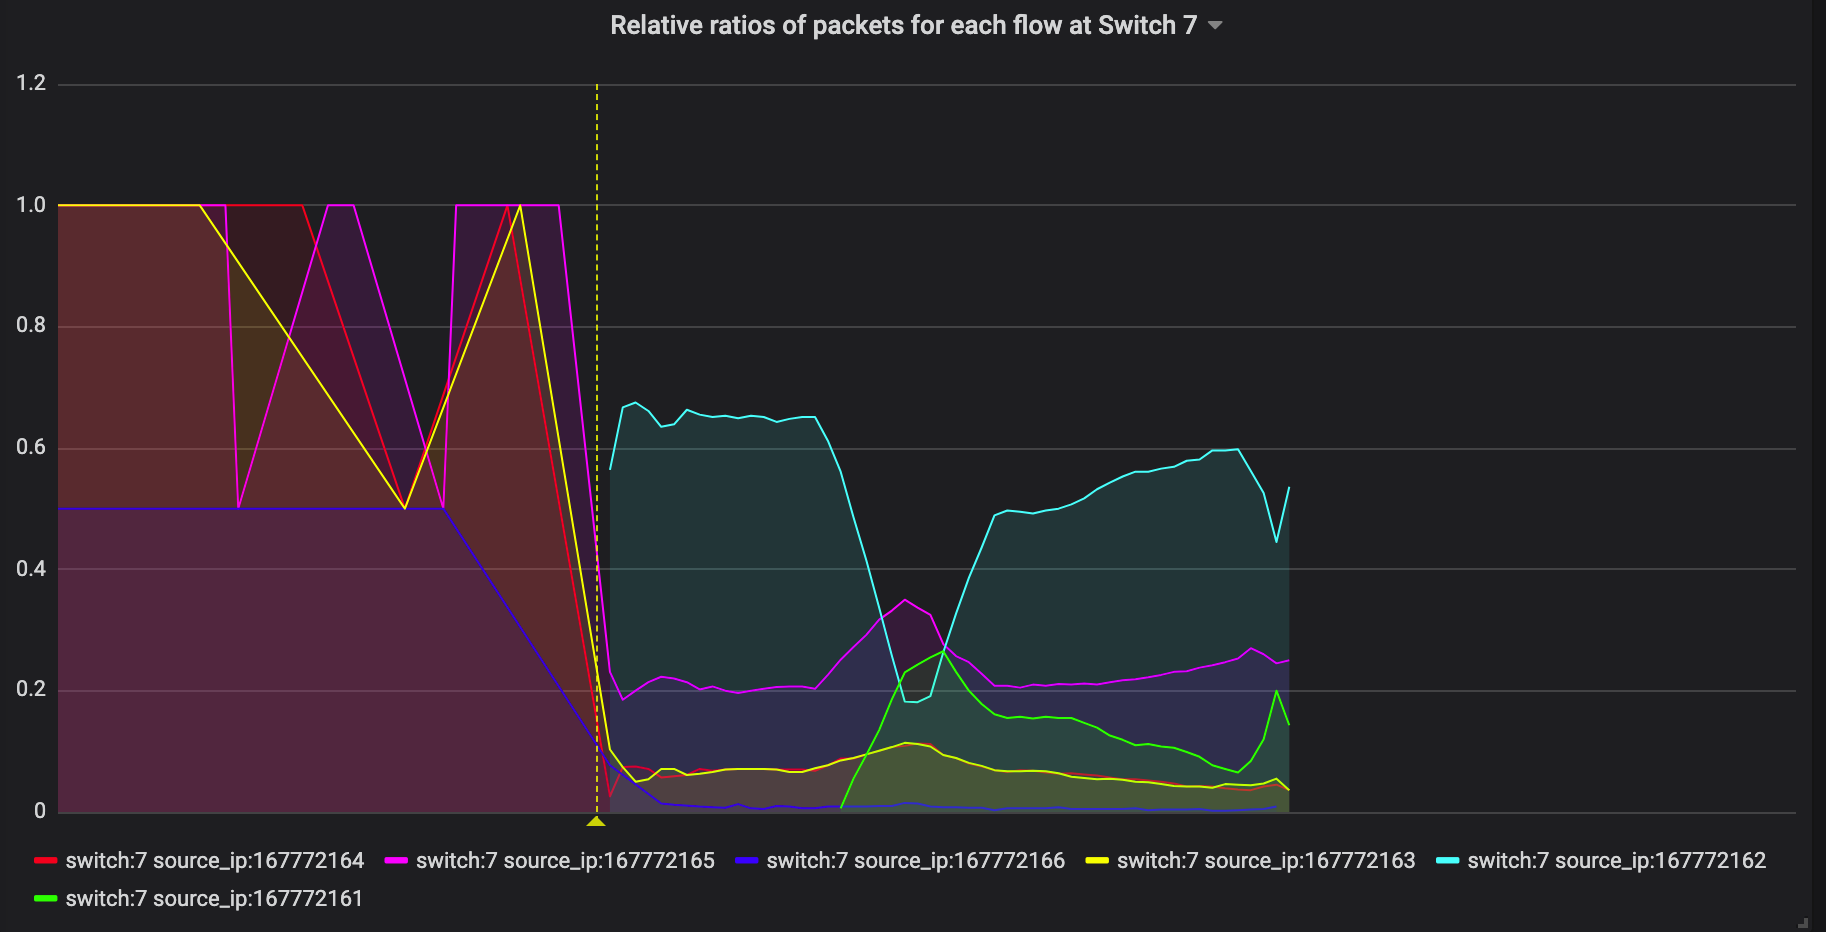
\includegraphics[width=1.0\columnwidth]{Figures/ratio_absolute.png}
		\rule{35em}{0.5pt}
	\caption[Relative Ratios]{Relative ratios for flows at a switch}
	\label{fig:QDAbsolute}
\end{figure}

\section{Ingress Throughputs for each flow in switch}

\subsection{Motivation}
This quantity captures the bandwidth of incoming flows in a switch at any point in time. This is the classical definition of bandwidth such that if, in an interval of time \emph{T},
\emph{p} number of packets of a flow enter the switch, then our plan is to compute \emph{packet size} * \emph{n} / \emph{T} for all flows
across all such intervals for a switch. We do this for all switches. Having a plot of this quantity will help us understand the distribution of incoming flows into a switch.

\subsection{Computation}
We use the following process for computing the quantity described above.

\begin{enumerate}
    \item Select an interval I which will serve as the window size for computing the throughput for a flow.
    \item For an interval \emph{ [Tleft - Tright]} in time, perform the following query on the Packetrecords table.
    \begin{verbatim}
    SELECT source_ip, COUNT(hash) 
    FROM packetrecords
    WHERE time_in > Tleft AND time_out > Tright
    GROUP BY source_ip;
    \end{verbatim}
    \item This query returns to us the list of flows that entered a switch in a particular time interval (as ensured by the WHERE clause) as well as the number of packets of
    each flow. The throughput for each flow can then be obtained by dividing the incoming number of bits (number of packets * packetsize) by the interval I (which is equal to the difference
    between Tleft and Tright).
    \item This query is then repeated at all I length intervals (by incrementing Tleft and Tright both by I each time) in the duration of the records of the switch.
\end{enumerate}

\subsection{Visual Result}
To show how a quantity like this will be helpful, refer to Fig. \ref{fig:Ing_Ind} and \ref{fig:Ing_Stacked} which represent the individual ingress throughputs as well as the stacked (sum of all) ingress throughput
for the switch. It can be seen that the ingress throughput is much more than 10 Gbps which is the capacity of the outgoing link, which is why the queue starts building up due to more packets
coming in than those being sent out for a particular interval.

\begin{figure}[htbp]
	\centering
		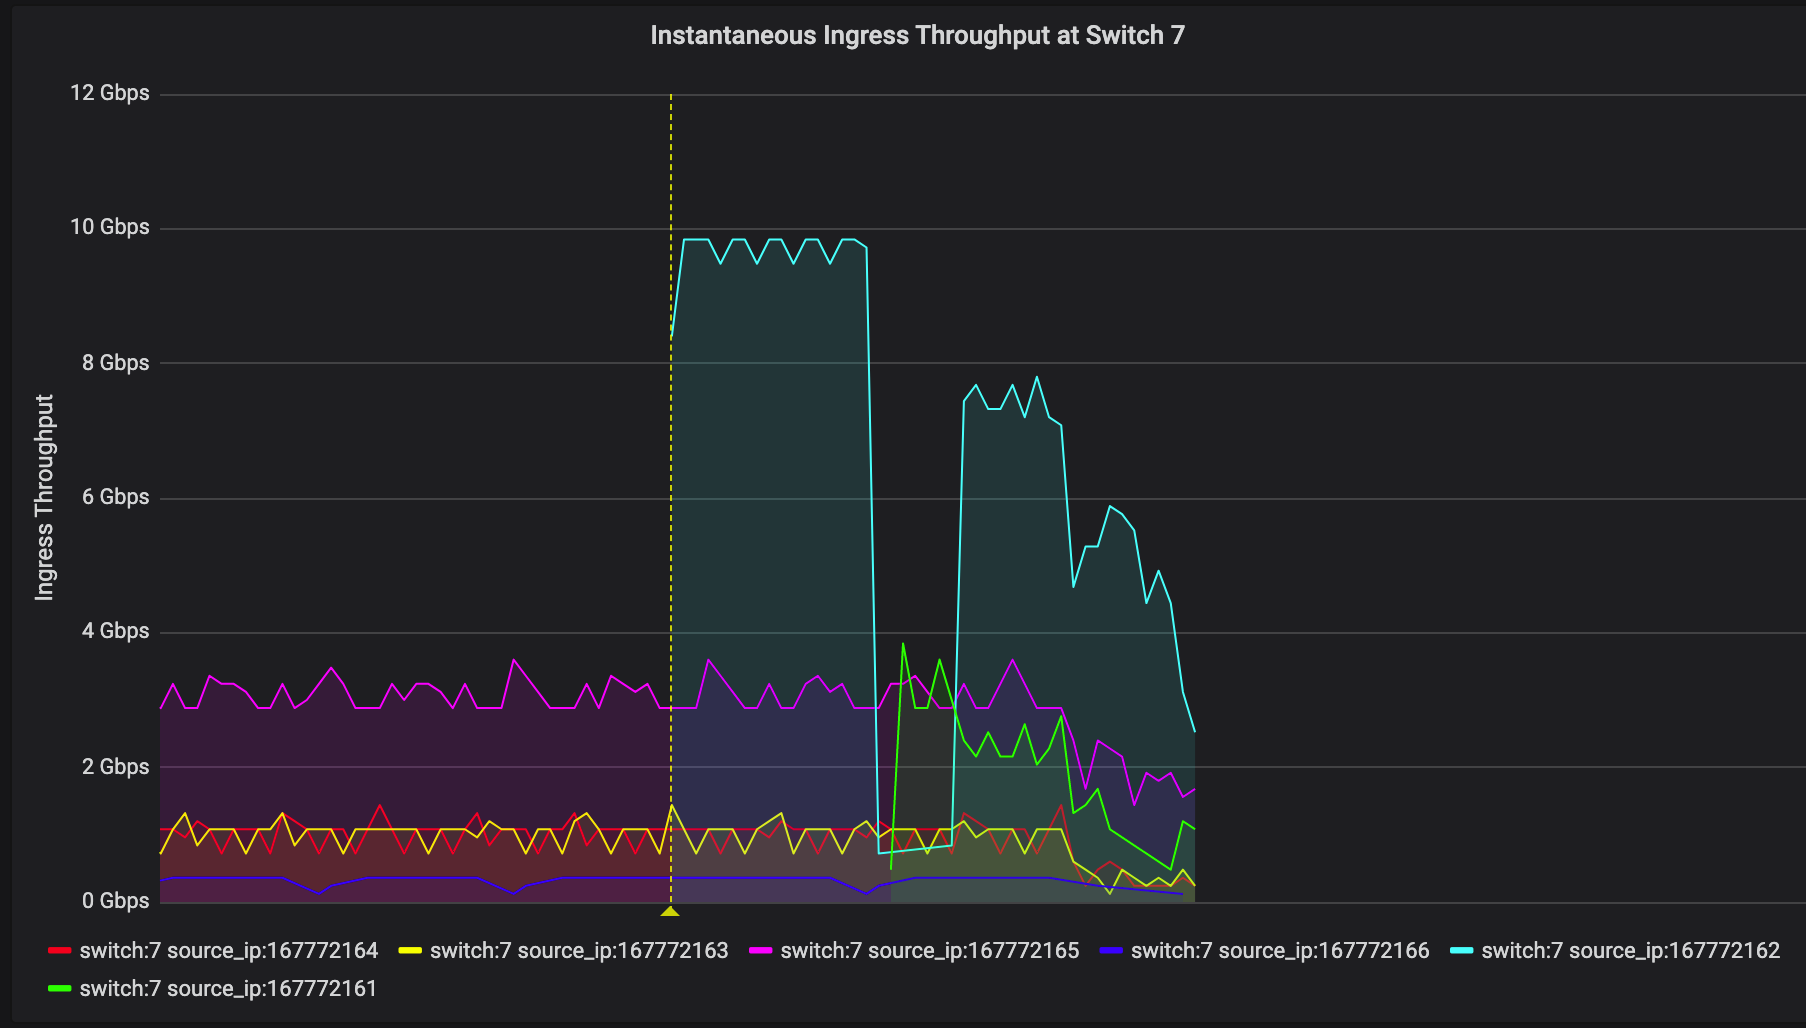
\includegraphics[width=1.0\columnwidth]{Figures/ingress_individual.png}
		\rule{35em}{0.5pt}
	\caption[Individual Ingress Throughputs]{Individual Ingress throughputs at switch}
	\label{fig:Ing_Ind}
\end{figure}

\begin{figure}[htbp]
	\centering
		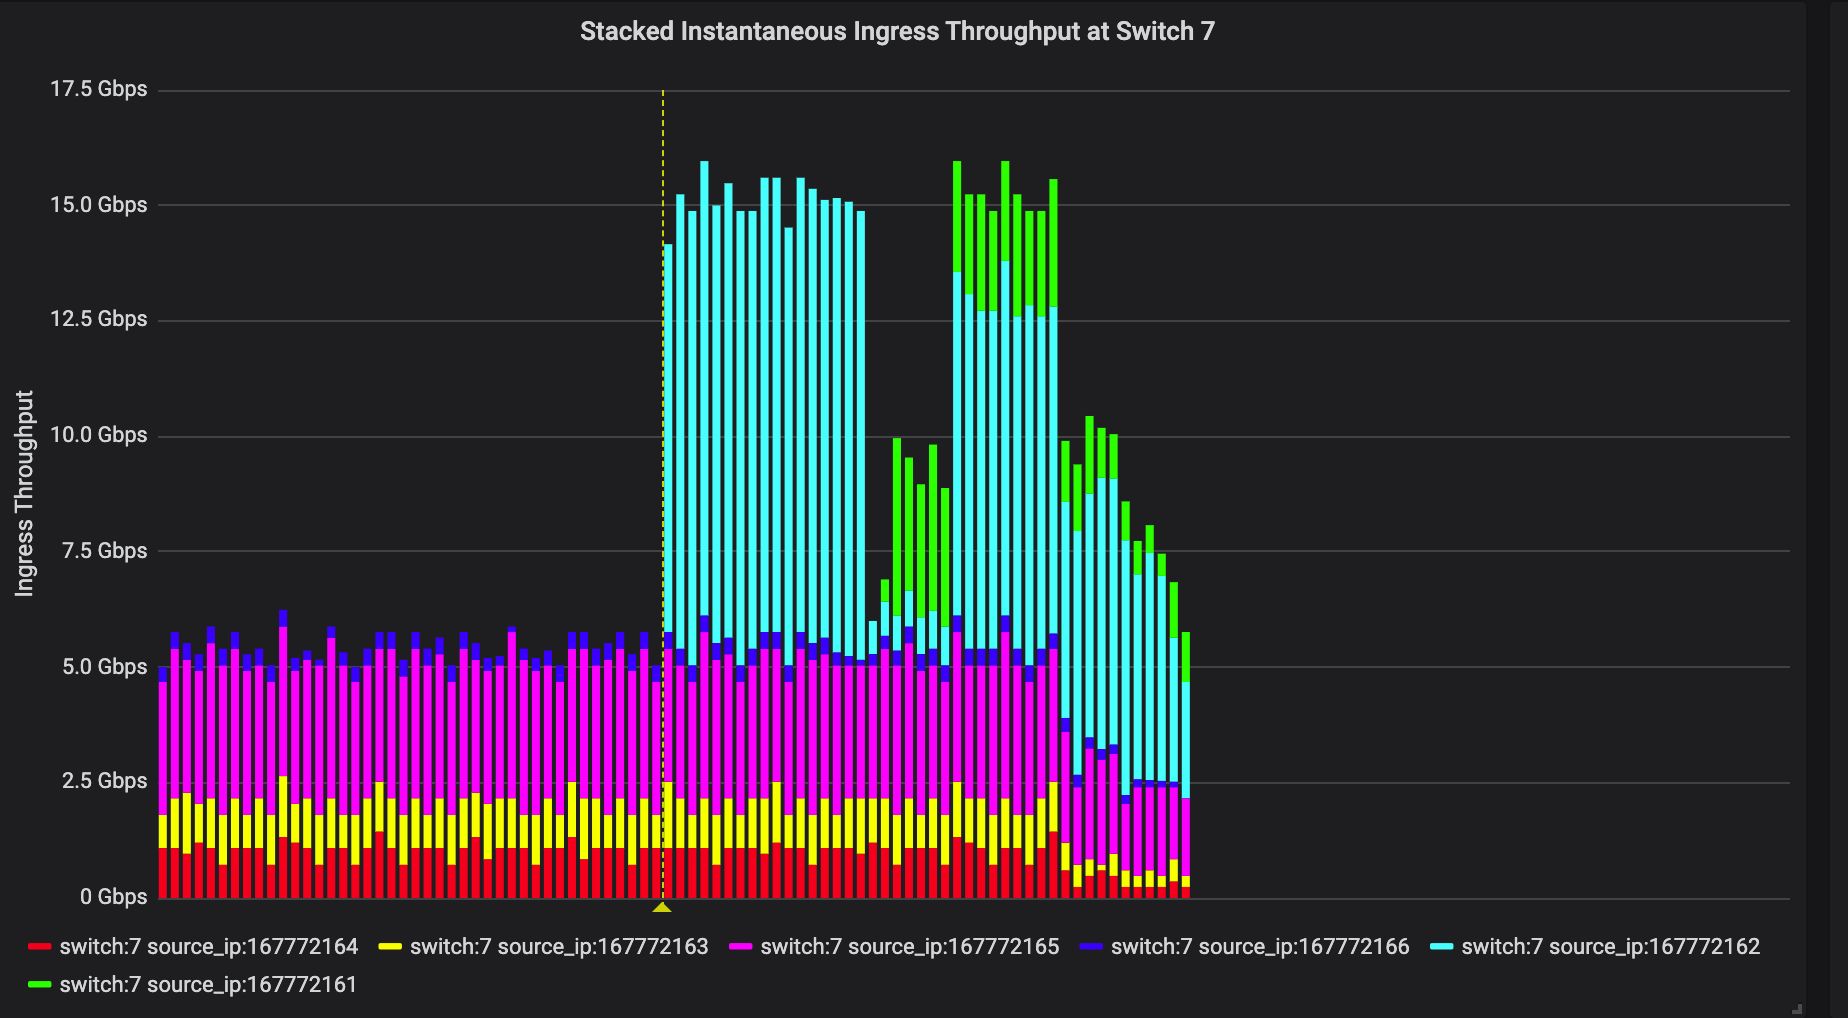
\includegraphics[width=1.0\columnwidth]{Figures/ingress_stacked.png}
		\rule{35em}{0.5pt}
	\caption[Stacked Ingress Throughputs]{Stacked Ingress throughputs at switch}
	\label{fig:Ing_Stacked}
\end{figure}

\section{Egress Throughputs for each link in network}

\subsection{Motivation}
This quantity captures the bandwidth at an interval of time for a link in the network. This is the most important quantity for creating a visualization that indicates
the bandwidth of all links at a particular point in time (Refer to Fig. \ref{})

\subsection{Computation}
The computation of bandwidth for all links in the network from the schema provided to us is a 2 step process. We firstly compute a table \emph{linkmaps} as described
below.

\begin{enumerate}
    \item Run the following query on MySQL via Python3
    \begin{verbatim}
    SELECT time_in, time_out, switch, hash
    FROM packetrecords
    ORDER BY hash, time_in;
    \end{verbatim}
    \item This query returns for us the records of a packet as it travels the network in a chronological manner. Thus if a packet visites switches S2, S3, S5, then we will
    obtain the records for that packet as captured by the switches in the order of the switch visited.
    \item From this data, we construct the table linkmaps containing the fields time enter (the timeout value of record at index i), time exit (the time in value of record at index i+1), from switch
    (the switch value of record at index i), to switch (the switch value of record at index i+1) and hash of the packet in question.
    \item Once we have constructed this linkmaps table, the process of calculating throughputs is relatively straightforward. We decide an interval I that will be the width for
    one calculation of throughput.
    \item We run the following query for a particular interval \emph{[Tleft - Tright]} for a particular switch S which we are considering as the source for links whose throughput we are calculating:
    \begin{verbatim}
    SELECT to_switch, time_exit 
    FROM linkmaps
    WHERE time_exit > Tleft AND time_exit < Tright AND from_switch = S
    GROUP BY to_switch;
    \end{verbatim}
    \item Now we collect all records going to a particular to switch, and calculate the throughput for that interval by dividing number of records times the packet size by the interval duration.
    This will be the throughput at a time (time exit) for the link represented by source as from switch and destination as to switch.
    \item This query is then repeated at all I length intervals (by incrementing Tleft and Tright both by I each time) in the duration of the records of linkmaps table.
\end{enumerate}

\subsection{Visual Result}
To show how a quantity like this will be helpful, refer to Fig. \ref{fig:Eg_Ind} the individual egress throughput on link connecting switch 9 and switch 7. It can be seen that the individual
egress throughput is constant at 10 Gbps which is the capacity of the outgoing link, showing that the link is being completely utilized.

This quantity is also extremely useful for creating visualizations like that in Fig. \ref{fig:Eg_example} which give a birds eye view of what exactly is happening in the network. This view
which can be changed over time, is invaluable for understanding what exactly happened in the network.

\begin{figure}[htbp]
	\centering
		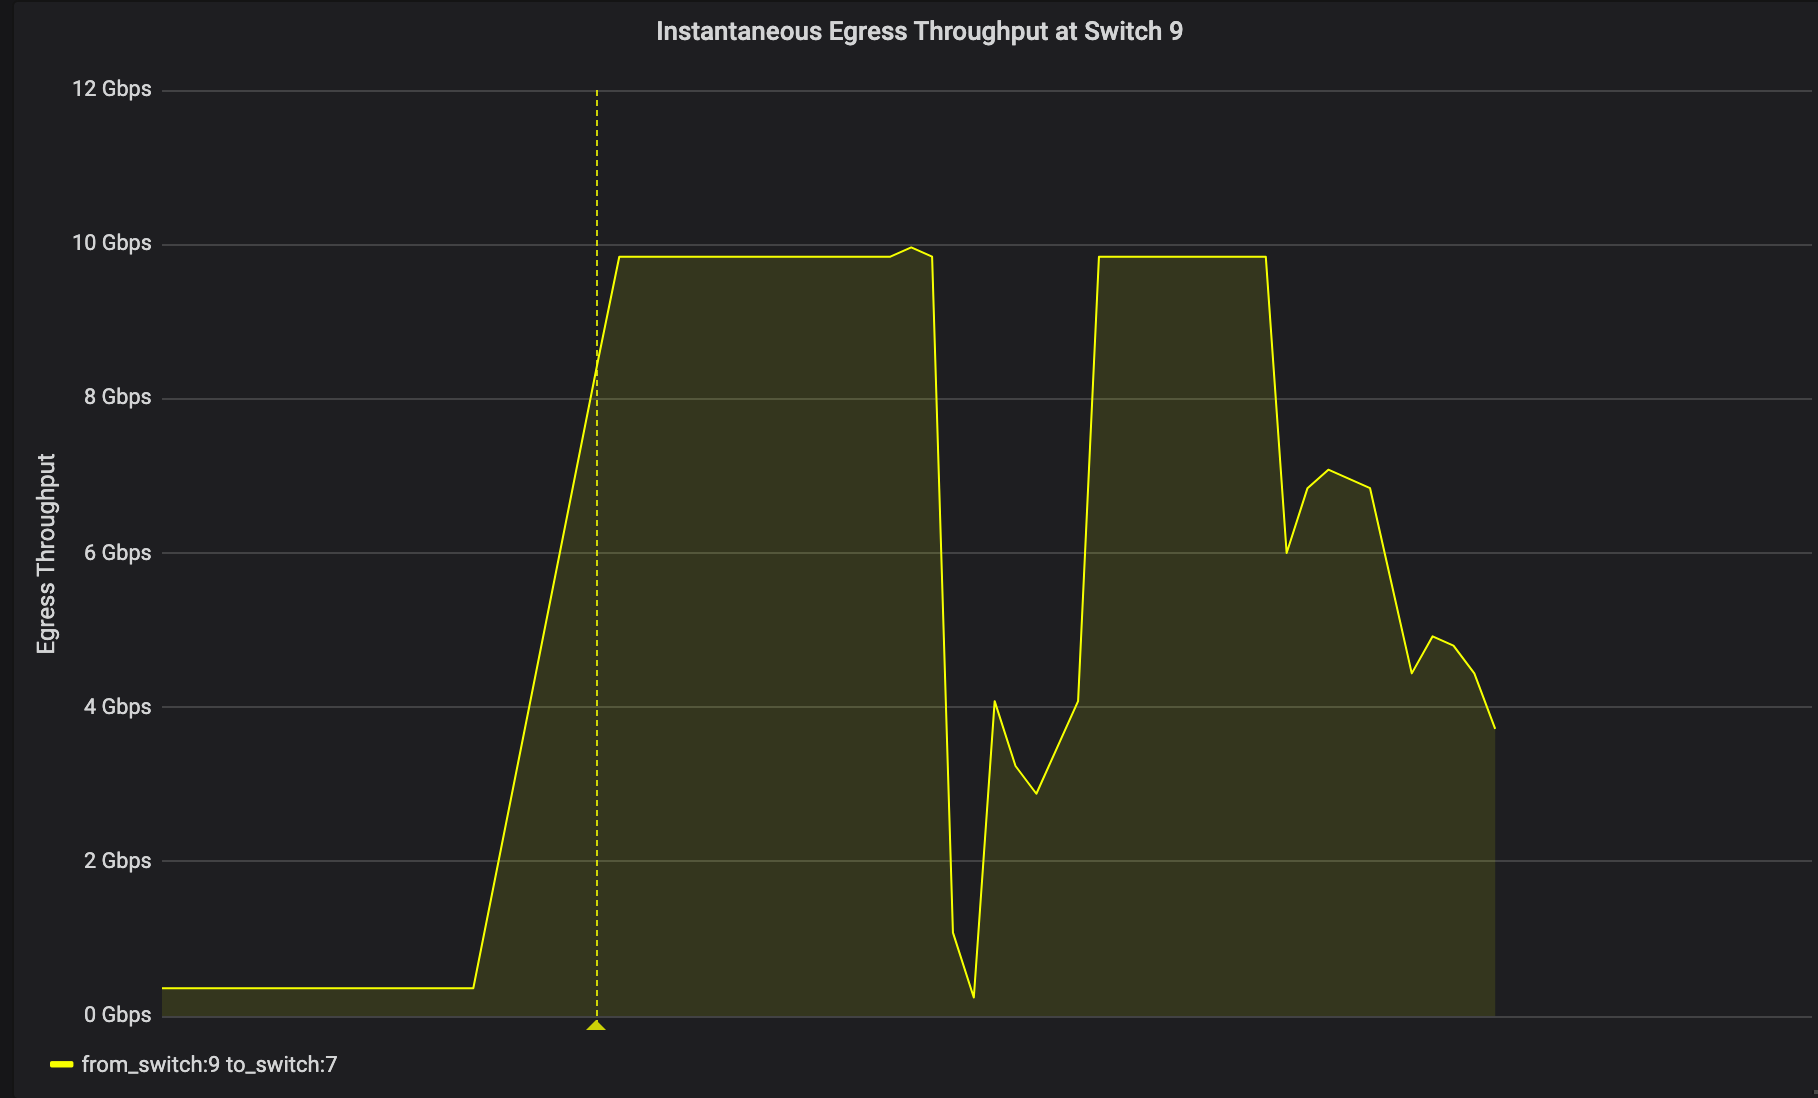
\includegraphics[width=1.0\columnwidth]{Figures/egress_individual.png}
		\rule{35em}{0.5pt}
	\caption[Individual Egress Throughputs]{Individual Engress throughput at switch}
	\label{fig:Eg_Ind}
\end{figure}

\begin{figure}[htbp]
	\centering
		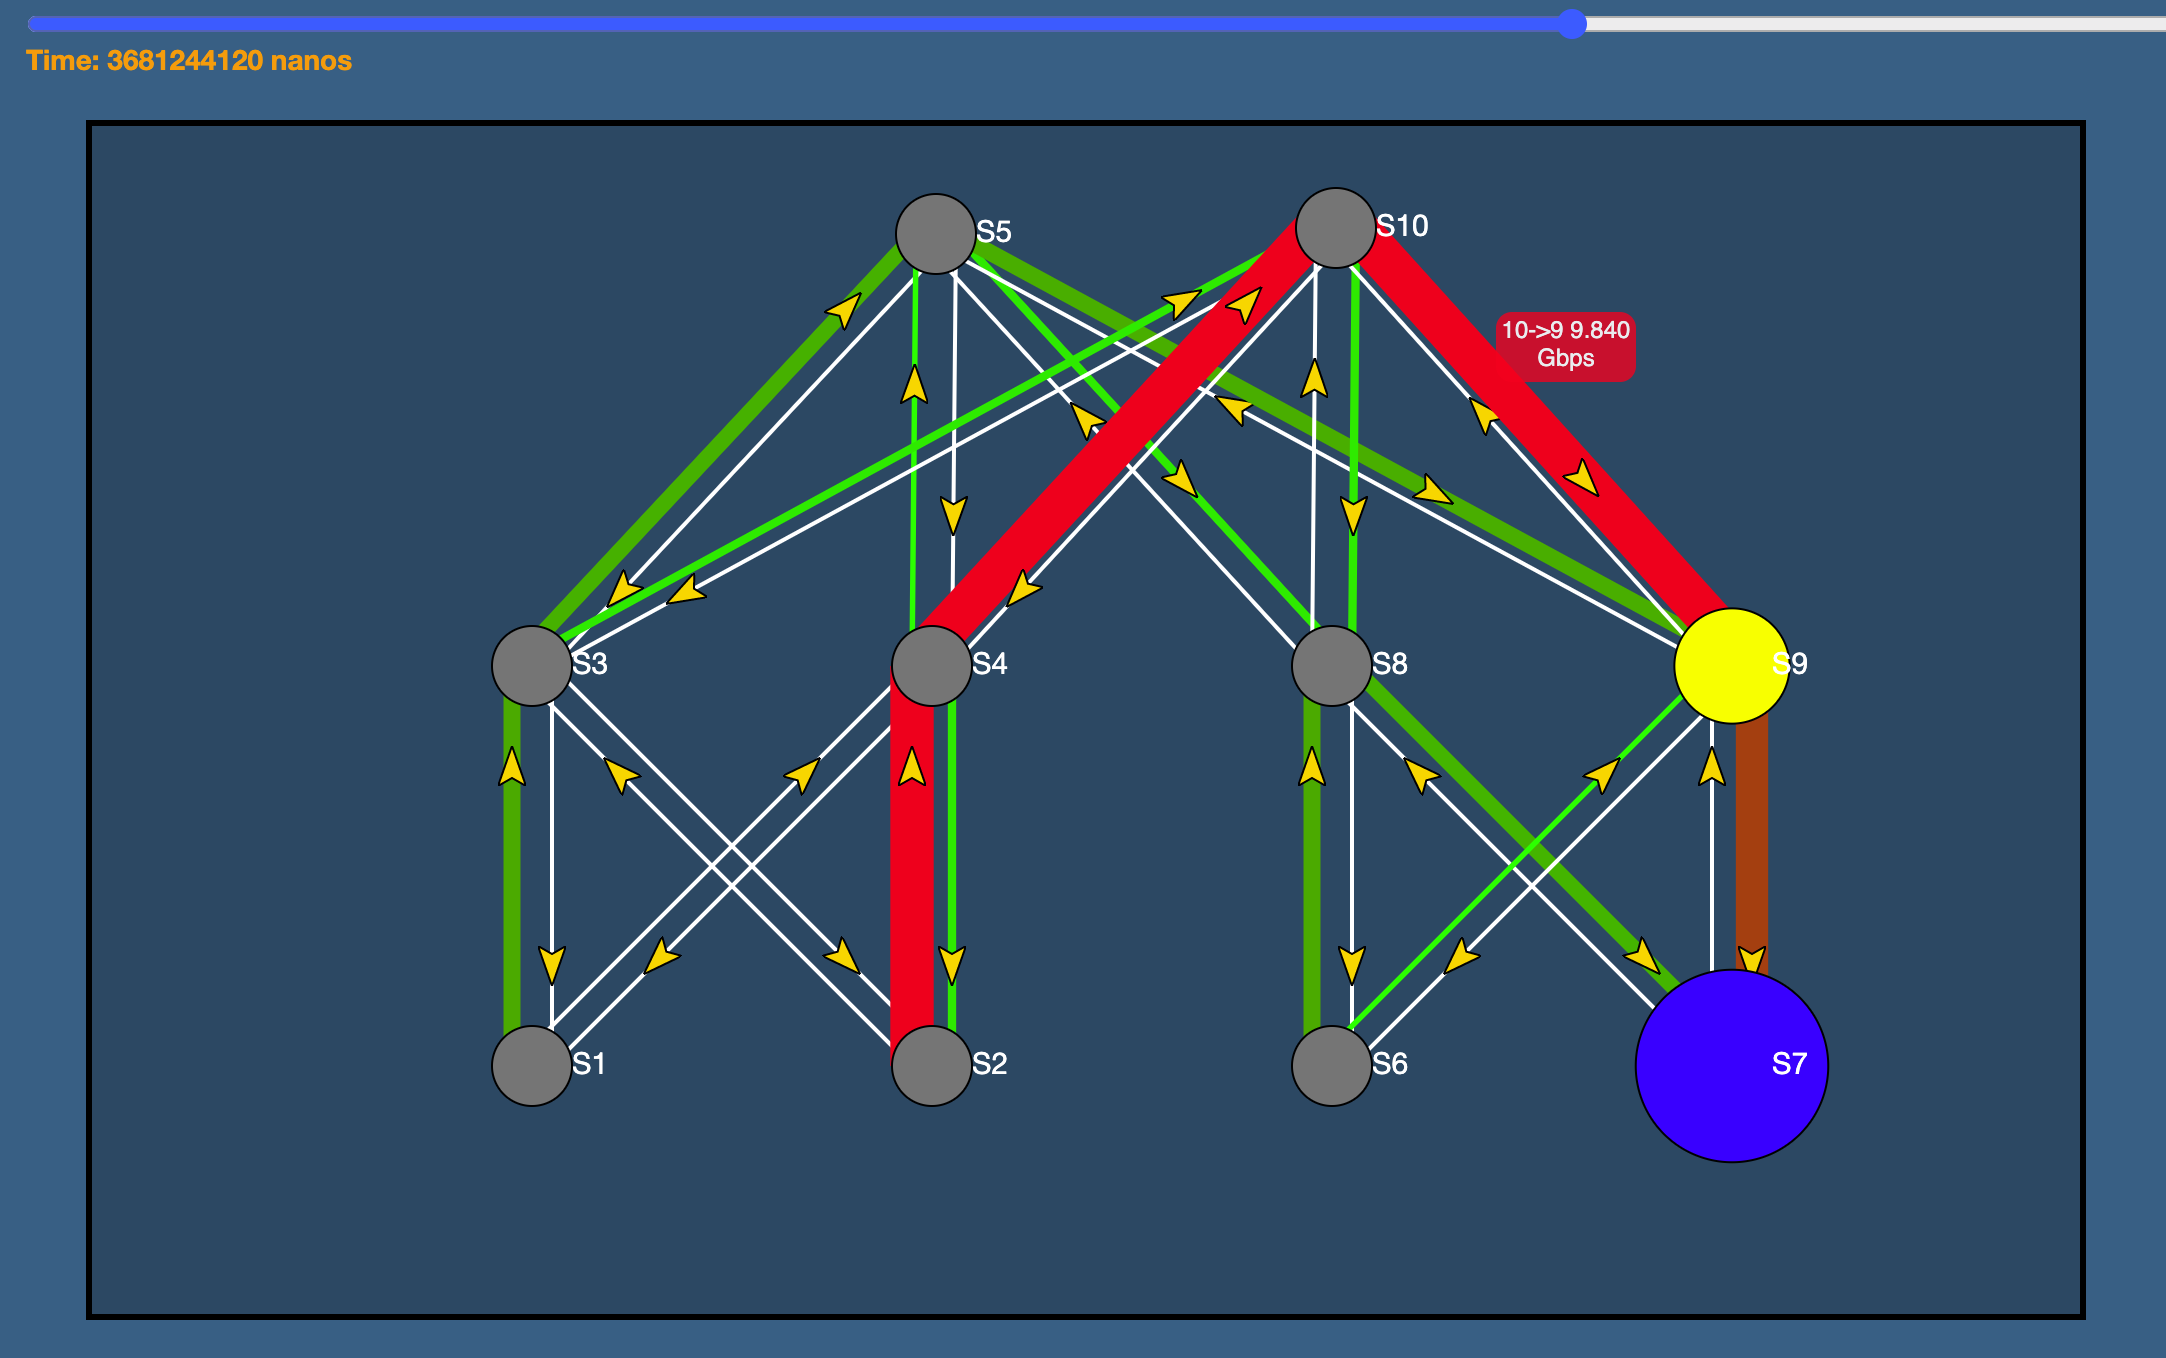
\includegraphics[width=1.0\columnwidth]{Figures/egress_example.png}
		\rule{35em}{0.5pt}
	\caption[Link Throughputs Visualizations]{An example of how powerful visualizations can be created with this quantity. The thick red link indicates existence of a heavy hitter flow dude to very high throughput. Then enlarged blue switch indicates buildup of queue in the switch.}
	\label{fig:Eg_example}
\end{figure}